\documentclass[11pt,a4paper]{article}
\usepackage[margin=2.5cm]{geometry}
\usepackage{amsmath,amssymb}
\usepackage{graphicx}
\usepackage{tcolorbox}
\usepackage{listings}
\usepackage{xcolor}
\usepackage{hyperref}
\usepackage{tikz}
\usetikzlibrary{shapes,arrows,chains}

% Color definitions
\definecolor{mlblue}{RGB}{0,102,204}
\definecolor{mlpurple}{RGB}{51,51,178}
\definecolor{mlorange}{RGB}{255,127,14}
\definecolor{mlgreen}{RGB}{44,160,44}

% Key concept box
\newtcolorbox{keybox}[1]{
  colback=mlblue!5!white,
  colframe=mlblue,
  fonttitle=\bfseries,
  title=#1
}

% Example box
\newtcolorbox{examplebox}[1]{
  colback=mlgreen!5!white,
  colframe=mlgreen,
  fonttitle=\bfseries,
  title=#1
}

% Code listing style
\lstset{
  basicstyle=\ttfamily\small,
  backgroundcolor=\color{gray!10},
  frame=single,
  numbers=left,
  numberstyle=\tiny\color{gray},
  breaklines=true,
  captionpos=b
}

\title{\textbf{Lecture Notes: Lesson 1}\\Blockchain Fundamentals}
\author{Cryptocurrency Course}
\date{}

\begin{document}

\maketitle

\tableofcontents
\newpage

\section{Introduction to Blockchain Technology}

\subsection{Historical Context}

The blockchain revolution began in 2008 with Satoshi Nakamoto's Bitcoin whitepaper titled \textit{"Bitcoin: A Peer-to-Peer Electronic Cash System"}. This groundbreaking work solved the long-standing double-spending problem without requiring a trusted third party.

\begin{keybox}{Key Innovation}
Blockchain technology enables \textbf{trustless consensus} in a distributed network. Participants can agree on the state of a shared ledger without trusting any single authority or intermediary.
\end{keybox}

\subsection{Core Characteristics}

Blockchain systems exhibit several fundamental properties:

\begin{itemize}
  \item \textbf{Decentralization}: No single point of control or failure
  \item \textbf{Immutability}: Historical records cannot be altered without detection
  \item \textbf{Transparency}: All transactions are visible to network participants
  \item \textbf{Security}: Cryptographic techniques protect data integrity
  \item \textbf{Consensus}: Agreement mechanisms ensure network-wide coordination
\end{itemize}

\section{Block Structure and Components}

\subsection{Anatomy of a Block}

Each block in a blockchain consists of two main parts: the \textbf{header} and the \textbf{body}.

\subsubsection{Block Header}

The header contains metadata that uniquely identifies and links the block:

\begin{enumerate}
  \item \textbf{Block Hash}: A unique identifier computed from all header fields
  \item \textbf{Previous Block Hash}: Links to the parent block, forming the chain
  \item \textbf{Timestamp}: When the block was created (Unix epoch time)
  \item \textbf{Nonce}: A variable used in the mining process (Proof-of-Work)
  \item \textbf{Merkle Root}: A cryptographic digest of all transactions in the block
\end{enumerate}

\begin{keybox}{Block Hash Formula}
The block hash is computed as:
\[
\text{BlockHash} = \text{SHA256}(\text{SHA256}(\text{Header}))
\]
This double-SHA256 provides additional security against potential collision attacks.
\end{keybox}

\subsubsection{Block Body}

The body contains the actual transaction data. In Bitcoin, a block can contain thousands of transactions. The Merkle root in the header provides a compact cryptographic summary of all these transactions.

\subsection{Mathematical Representation}

We can formally define a block $B_i$ as:
\[
B_i = (H_i, T_i)
\]
where:
\begin{itemize}
  \item $H_i$ is the header containing: $\{h_{i-1}, t_i, n_i, m_i\}$
  \item $h_{i-1}$ is the hash of the previous block
  \item $t_i$ is the timestamp
  \item $n_i$ is the nonce
  \item $m_i$ is the Merkle root
  \item $T_i = \{tx_1, tx_2, \ldots, tx_k\}$ is the set of transactions
\end{itemize}

\section{Cryptographic Hash Functions}

\subsection{Properties of Hash Functions}

A cryptographic hash function $H: \{0,1\}^* \rightarrow \{0,1\}^n$ must satisfy:

\begin{enumerate}
  \item \textbf{Deterministic}: Same input always produces same output
  \item \textbf{Fast Computation}: $H(m)$ can be computed quickly
  \item \textbf{Pre-image Resistance}: Given $h$, it's infeasible to find $m$ such that $H(m) = h$
  \item \textbf{Second Pre-image Resistance}: Given $m_1$, it's infeasible to find $m_2 \neq m_1$ such that $H(m_1) = H(m_2)$
  \item \textbf{Collision Resistance}: It's infeasible to find any pair $(m_1, m_2)$ such that $H(m_1) = H(m_2)$
  \item \textbf{Avalanche Effect}: Small input changes produce dramatically different outputs
\end{enumerate}

\begin{examplebox}{SHA-256 Example}
Consider two similar inputs:
\begin{lstlisting}[language=Python]
import hashlib

# Original input
input1 = "Hello World"
hash1 = hashlib.sha256(input1.encode()).hexdigest()
print(f"Hash 1: {hash1}")

# Slightly modified input
input2 = "Hello world"  # lowercase 'w'
hash2 = hashlib.sha256(input2.encode()).hexdigest()
print(f"Hash 2: {hash2}")
\end{lstlisting}

Output:
\begin{verbatim}
Hash 1: a591a6d40bf420404a011733cfb7b190d62c65bf0bcda32b57b277d9ad9f146e
Hash 2: 64ec88ca00b268e5ba1a35678a1b5316d212f4f366b2477232534a8aeca37f3c
\end{verbatim}

Notice: A single character change produces a completely different hash!
\end{examplebox}

\subsection{SHA-256 Algorithm Overview}

SHA-256 (Secure Hash Algorithm 256-bit) processes data in 512-bit blocks:

\begin{enumerate}
  \item \textbf{Preprocessing}: Pad message to multiple of 512 bits
  \item \textbf{Initialize Hash Values}: Eight 32-bit words (constants)
  \item \textbf{Process Message Blocks}: 64 rounds of operations per block
  \item \textbf{Output}: Final 256-bit hash value
\end{enumerate}

The algorithm uses logical functions (AND, OR, XOR, NOT), bitwise rotation, and modular addition to achieve strong cryptographic properties.

\section{Hash Chain and Blockchain Linkage}

\subsection{Chain Formation}

The blockchain's immutability comes from its hash chain structure. Each block contains the hash of its predecessor, creating a cryptographic link:

\[
B_0 \xrightarrow{h_0} B_1 \xrightarrow{h_1} B_2 \xrightarrow{h_2} B_3 \xrightarrow{h_3} \cdots
\]

\begin{keybox}{Immutability Proof}
If an attacker modifies any transaction in block $B_i$:
\begin{enumerate}
  \item The Merkle root $m_i$ changes
  \item The block hash $h_i$ changes
  \item Block $B_{i+1}$ now has an invalid previous hash reference
  \item All subsequent blocks must be recomputed
  \item The attacker must redo all Proof-of-Work for blocks $i$ through $n$
  \item This becomes computationally infeasible for deeply buried blocks
\end{enumerate}
\end{keybox}

\subsection{Genesis Block}

The first block in the chain (Block 0) has no predecessor. It's called the \textbf{genesis block} and is typically hardcoded into the blockchain software.

Bitcoin's genesis block (January 3, 2009) includes the famous message:
\begin{quote}
\textit{"The Times 03/Jan/2009 Chancellor on brink of second bailout for banks"}
\end{quote}

\section{Merkle Trees}

\subsection{Structure and Purpose}

A Merkle tree is a binary tree of hashes used to efficiently summarize and verify large data sets.

\subsubsection{Construction Algorithm}

\begin{enumerate}
  \item Hash each transaction: $H(tx_1), H(tx_2), \ldots, H(tx_n)$
  \item Pair hashes and concatenate: $H(H(tx_1) || H(tx_2))$
  \item Continue until single root hash remains
  \item If odd number of leaves, duplicate the last hash
\end{enumerate}

\begin{examplebox}{Merkle Tree Construction}
For 4 transactions A, B, C, D:

\begin{verbatim}
                    Root = H(ABCD)
                   /              \
            H(AB)                    H(CD)
           /     \                  /     \
        H(A)     H(B)            H(C)     H(D)
         |        |               |        |
        Tx A     Tx B            Tx C     Tx D
\end{verbatim}

Python implementation:
\begin{lstlisting}[language=Python]
import hashlib

def hash_pair(a, b):
    """Hash concatenation of two values"""
    return hashlib.sha256((a + b).encode()).hexdigest()

def build_merkle_root(transactions):
    """Build Merkle root from list of transactions"""
    if len(transactions) == 0:
        return None
    if len(transactions) == 1:
        return hashlib.sha256(transactions[0].encode()).hexdigest()

    # Hash all transactions
    level = [hashlib.sha256(tx.encode()).hexdigest()
             for tx in transactions]

    # Build tree bottom-up
    while len(level) > 1:
        next_level = []
        for i in range(0, len(level), 2):
            if i + 1 < len(level):
                next_level.append(hash_pair(level[i], level[i+1]))
            else:
                # Odd number: duplicate last hash
                next_level.append(hash_pair(level[i], level[i]))
        level = next_level

    return level[0]
\end{lstlisting}
\end{examplebox}

\subsection{Merkle Proofs}

Merkle trees enable efficient proof of inclusion. To prove a transaction is in a block, you only need:
\begin{itemize}
  \item The transaction itself
  \item $\log_2(n)$ sibling hashes (the Merkle path)
  \item The Merkle root from the block header
\end{itemize}

\textbf{Complexity}: For a block with 2048 transactions, you need only 11 hashes to prove inclusion (versus downloading all 2048 transactions).

\section{Consensus Mechanisms}

\subsection{The Byzantine Generals Problem}

Blockchain consensus solves a classic distributed systems problem: how can nodes agree on a single truth when some nodes may be malicious or faulty?

\subsection{Proof-of-Work (PoW)}

\subsubsection{Mining Process}

Miners compete to find a nonce such that:
\[
H(\text{header}) < \text{target}
\]

The target determines difficulty. Lower target = harder problem.

\begin{keybox}{Difficulty Adjustment}
Bitcoin adjusts difficulty every 2016 blocks to maintain approximately 10-minute block time:
\[
\text{new\_difficulty} = \text{old\_difficulty} \times \frac{\text{expected\_time}}{\text{actual\_time}}
\]
where expected time = $2016 \times 10$ minutes.
\end{keybox}

\subsubsection{Security Analysis}

An attacker needs $>50\%$ of network hash rate to:
\begin{itemize}
  \item Consistently outpace honest miners
  \item Rewrite transaction history
  \item Double-spend coins
\end{itemize}

\textbf{Cost}: Bitcoin's hash rate (as of 2024) exceeds 400 EH/s, making attacks economically infeasible.

\subsection{Proof-of-Stake (PoS)}

\subsubsection{Core Concept}

Validators are chosen to propose blocks based on their stake (coins locked as collateral).

Selection probability:
\[
P(\text{validator } i) \propto \text{stake}_i
\]

\subsubsection{Advantages}
\begin{itemize}
  \item Energy efficient (no computational waste)
  \item Slashing: Malicious validators lose their stake
  \item Lower barrier to entry
\end{itemize}

\subsubsection{Challenges}
\begin{itemize}
  \item \textbf{Nothing-at-Stake}: Validators can vote on multiple forks without cost
  \item \textbf{Long-Range Attacks}: Attackers with past stakes can rewrite history
  \item Solutions: Checkpointing, slashing conditions
\end{itemize}

\subsection{Comparison Table}

\begin{center}
\begin{tabular}{|l|l|l|}
\hline
\textbf{Feature} & \textbf{Proof-of-Work} & \textbf{Proof-of-Stake} \\
\hline
Energy Use & Very High & Low \\
Security Basis & Computational power & Economic stake \\
Entry Barrier & Hardware cost & Token purchase \\
51\% Attack Cost & Rent/buy 51\% hash rate & Own 51\% of supply \\
Finality & Probabilistic & Fast/deterministic \\
Examples & Bitcoin, Litecoin & Ethereum 2.0, Cardano \\
\hline
\end{tabular}
\end{center}

\section{Decentralization Principles}

\subsection{Network Topology}

Blockchain networks use peer-to-peer (P2P) architecture where:
\begin{itemize}
  \item Each node maintains a full or partial copy of the ledger
  \item Nodes communicate directly without central coordination
  \item Transaction propagation uses gossip protocol
\end{itemize}

\subsection{Benefits of Decentralization}

\begin{enumerate}
  \item \textbf{Censorship Resistance}: No single entity can block transactions
  \item \textbf{Fault Tolerance}: Network survives individual node failures
  \item \textbf{Reduced Trust Requirements}: Cryptography replaces institutional trust
  \item \textbf{Transparency}: All participants can audit the system
\end{enumerate}

\subsection{Decentralization Trilemma}

Vitalik Buterin identified three desirable properties that are difficult to achieve simultaneously:

\begin{center}
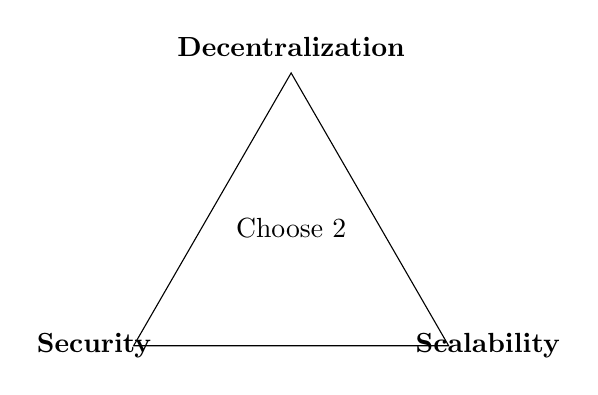
\begin{tikzpicture}
  \draw (0,0) -- (4,0) -- (2,3.464) -- cycle;
  \node at (2,3.8) {\textbf{Decentralization}};
  \node at (-0.5,0) {\textbf{Security}};
  \node at (4.5,0) {\textbf{Scalability}};
  \node at (2,1.5) {Choose 2};
\end{tikzpicture}
\end{center}

Trade-offs are inevitable; different blockchains optimize different corners of this triangle.

\section{Study Questions}

\subsection{Conceptual Questions}

\begin{enumerate}
  \item Explain why changing a single transaction in block 100 would invalidate all subsequent blocks.
  \item How does the Merkle root enable lightweight clients to verify transactions?
  \item Compare the security models of Proof-of-Work versus Proof-of-Stake.
  \item What prevents a miner from including invalid transactions in a block?
  \item Describe the avalanche effect and its importance in cryptographic hashing.
\end{enumerate}

\subsection{Computational Problems}

\begin{enumerate}
  \item Given transactions [A, B, C, D, E, F, G, H], draw the complete Merkle tree and calculate the root hash (use simplified hash function for demonstration).

  \item If Bitcoin's current difficulty requires finding a hash starting with 19 leading zeros, what is the approximate probability of success for a single hash attempt?

  \item A blockchain has 100,000 blocks with 2000 transactions each. How many hashes are needed for a Merkle proof of inclusion?

  \item Calculate the new difficulty if the last 2016 blocks took 18,000 minutes instead of the expected 20,160 minutes.
\end{enumerate}

\subsection{Implementation Exercises}

\begin{enumerate}
  \item Implement a simple blockchain with basic block structure (header + body).
  \item Create a function to validate the hash chain integrity.
  \item Build a Merkle tree implementation with proof generation and verification.
  \item Simulate a basic Proof-of-Work mining process with adjustable difficulty.
\end{enumerate}

\section{Further Reading}

\begin{itemize}
  \item Nakamoto, S. (2008). \textit{Bitcoin: A Peer-to-Peer Electronic Cash System}.
  \item Antonopoulos, A. M. (2017). \textit{Mastering Bitcoin: Programming the Open Blockchain}.
  \item Narayanan, A., et al. (2016). \textit{Bitcoin and Cryptocurrency Technologies}.
  \item Ethereum Foundation. (2023). \textit{Ethereum Whitepaper and Yellowpaper}.
  \item Buterin, V. (2017). \textit{The Blockchain Scalability Trilemma}.
\end{itemize}

\end{document}
